\documentclass[../document.tex]{subfiles}

\begin{document}
	\subsection{Сравнительный анализ аналогичных решений}
	\par В результате проведённого анализа рынка было обнаружено большое количество сервисов A/B тестирования, большинство из которых предоставляют свои услуги в формате software-as-a-service. Большинство таких сервисов предлагают не только A/B тестирование, но и аналитику вообще; некоторые предлагают создание A/B тестов в визуальном конструкторе, где веб-страница меняется вручную, без написания кода. Интеграция этих систем из-за использования встроенной аналитики потребовала бы большого количества рабочего времени со стороны разработчиков <<Дрома>>.
	\par Google Optimize и Firebase A/B Testing \cite{optimize, firebase} доступны бесплатно и входят в состав Google Analytics и Firebase соответственно. Очевидным преимуществом является то, что эти сервисы уже использовались на <<Дроме>>, и, поэтому, не требовали больших усилий на их интеграцию.
	\par Optimizely \cite{optimizely} --- это ещё один из ведущих сервисов веб и мобильной аналитики, который, наоборот, вырос из сервиса для A/B тестирования.
	\par VWO \cite{vwo} --- также одна из ведущих коммерческих систем, по своему функционалу значимо не отличающаяся от Optimizely.
	\par Evergage \cite{evergage} --- платформа аналитики, позволяющая проводить A/B тесты.
	\par Taplytics \cite{taplytics} --- платформа аналитики с on-premises вариантом, со встроенным функционалом A/B тестирования.
	\par Countly \cite{countly} --- система аналитики с открытым исходным кодом. A/B тестирование --- платный плагин с коммерческой лицензией. Данные событий хранятся в MongoDB, что не подходит для наших объёмов данных.
	\par Matomo \cite{matomo} --- система аналитики с открытым исходным кодом. A/B тестирование --- платный плагин с коммерческой лицензией. Данные событий хранятся в MySQL, что не подходит для наших объёмов данных.
	\par Также было обнаружено несколько полностью свободных решений.
	\par Planout \cite{planout} --- решение от Facebook. Поддерживает разделение пользователей по когортам по достаточно сложным правилам, но не содержит функционала анализа результатов.
	\par Sixpack \cite{sixpack} --- решение от SeatGeek. Делит пользователей на когорты и подсчитывает конверсию для вариантов.
	\par Подробное сравнение аналогов по сформулированным требованиям представлено в таблице \ref{table:comparsion}.
 	\begin{fefutable}[h]{|p{8cm}|c|c|c|c|c|c|c|c|c|}{\label{table:comparsion}Сравнительный анализ аналогичных решений}
		\hline
		& \rot{Google\ } & \rot{Optimizely\ } & \rot{VWO\ } & \rot{Evergage\ } & \rot{Taplytics\ } & \rot{Countly\ } & \rot{Matomo\ } & \rot{Planout\ } & \rot{Sixpack\ }\\
		\hline
		возможность проводить A/B тесты как в мобильных приложениях, так и на сайте & 
		\textpm & + & + & + & + & + & + & \textminus & \textminus \\
		\hline
		возможность самостоятельной поддержки (доработки) системы &
		\textminus & \textminus & \textminus & \textminus & \textminus & + & + & + & + \\
		\hline
		возможность анализа сырых данных &
		+ & \textpm & \textpm & + & + & \textpm & \textpm & \textminus & \textminus \\
		\hline
		гибкая настройка метрики А/Б теста &
		\textminus & \textminus & \textminus & \textminus & \textminus & \textminus & \textminus & \textminus & \textminus \\
		\hline 
		хостинг системы на своих серверах &
		\textminus & \textminus & \textminus & \textminus & + & + & + & + & + \\
		\hline
		использование корректных статистических методов &
		+ & + & + & + & + & + & \textminus & \textminus & \textminus \\
		\hline
		использование методик уменьшения дисперсии &
		\textminus & \textminus & \textminus & \textminus & \textminus & \textminus & \textminus & \textminus & \textminus \\
		\hline
		возможность работы с уже существующими на <<Дроме>> базами данных &
		\textminus & \textminus & \textminus & \textminus & \textminus & \textminus & \textminus & \textminus & \textminus \\
		\hline
	\end{fefutable}
	\par Таким образом, ни одно из представленных на данный момент на рынке решений не удовлетворяет всем сформулированным требованиям, поэтому целесообразна разработка собственного решения.
	\subsection{Инфраструктура <<Дрома>>}
	\par Большую часть того, как должна быть устроена система, определяют уже существующие внутри <<Дрома>> программные решения.
	\par Так, в компании нет единой системы аналитики, и для большинства метрик требуется забирать сразу из нескольких источников. Как правило, это различные сервера СУБД MySQL и Clickhouse, а также REST API.
	\par Управление A/B тестами уже осуществляется через админ-панель A/B тестов или Firebase, поэтому необходимость в данном функционале в разрабатываемой системе отсутствует.
	\par По этой причине основными задачами системы являются определение метрик и подведение результатов A/B тестов, а не непосредственно управление A/B тестами. При этом каждая метрика задаётся кодом на ЯП Python, что обеспечивает практически неограниченную гибкость.
	\subsection{Требования к окружению}
	\subsubsection{Требования к аппаратному обеспечению}
	\par Развёртывание системы происходило в Kubernetes, со следующими параметрами:
	\begin{itemize}
		\item 2 vCPU;
		\item 4 ГБ оперативной памяти;
		\item 1 ГБ места на диске.
	\end{itemize}
	\subsubsection{Требования к программному обеспечению}
	\par Так как система разрабатывалась с применением технологий виртуализации, то единственным требованием является Kubernetes версии 1.16.3 или совместимый с ней.
	\subsubsection{Требования к пользователю}
	\begin{itemize}
		\item Понимание принципов и целей A/B тестирования;
		\item Умение правильно выбрать метрику для A/B теста;
		\item Умение работать с браузером и веб-приложениями.
	\end{itemize}
	\subsection{Спецификация данных}
	\par На рисунке \ref{image:db_plot} схематически изображена структура базы данных, используемая системой.
	\par Формат данных, обрабатываемых системой, не описывается из-за большого количества различных вариантов.
	\begin{figure}[h] 
		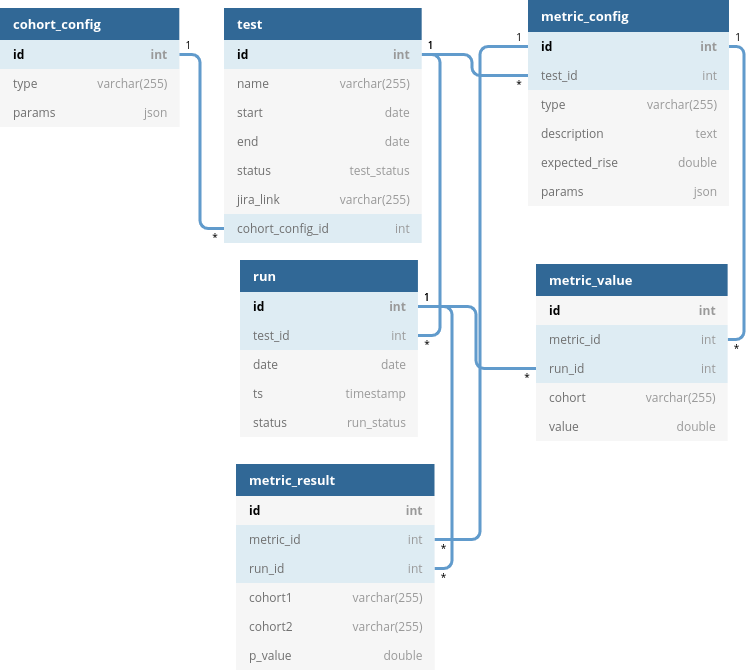
\includegraphics[width=\linewidth]{A_B v.3.0.png}
		\caption{\label{image:db_plot}Структура базы данных}
	\end{figure}
	\subsection{Требования к интерфейсу}
	\par Интерфейс системы должен позволять:
	\begin{enumerate}
		\item Создавать A/B тесты;
		\item Изменять созданные A/B тесты;
		\item Останавливать тесты;
		\item Просматривать список тестов;
		\item Просматривать результаты как текущих, так и завершённых тестов.
	\end{enumerate}
	\par При этом интерфейс должен быть:
	\begin{enumerate}
		\item Графическим;
		\item Доступным через веб-браузер.
	\end{enumerate}
\end{document}